\documentclass[12pt]{article}

\usepackage{url} % websites in bib
\usepackage{hyperref}
\usepackage[a4paper,left=1in,right=1in,top=1in,bottom=1in]{geometry} % margins
\usepackage{paralist} % compact enumerates

\usepackage{graphicx}
\usepackage{caption}
\usepackage{subcaption}

\usepackage{amsmath}

\begin{document}
	\title{}
	\author{Stefan Sebastian, 242}
	\date{}
	\maketitle
	
	\begin{abstract}
	
	\end{abstract}

	\newpage
	\tableofcontents
	\newpage
	
	\section{Dataset}
	The dataset used for this experiment is a collection of beer reviews taken from the BeerAdvocate website. The original dataset was made up out of 1.5 million user reviews, from 33387 different users, collected between 1998 and 2011. It is not available at this time but I found a subset of around 500 thousand reviews on data.world\cite{BeerAdvocateData}. 
	
	The data is in csv format, each row containing various information like: beer name, beer style, alcohol content, scores for taste, appearance, aroma and a textual review. The only columns considered for this experiment were the beer style and the text review.
	
	On exploratory data analysis, 407 duplicate and 119 missing reviews were found. Also there are 104 distinct beer styles and the amount of data for each of them is quite imbalanced as can be see in figure \ref{fig:initialDistribution}, where each bar represents a beer style with a size proportional to the number of reviews for it.
	
	\begin{figure}
		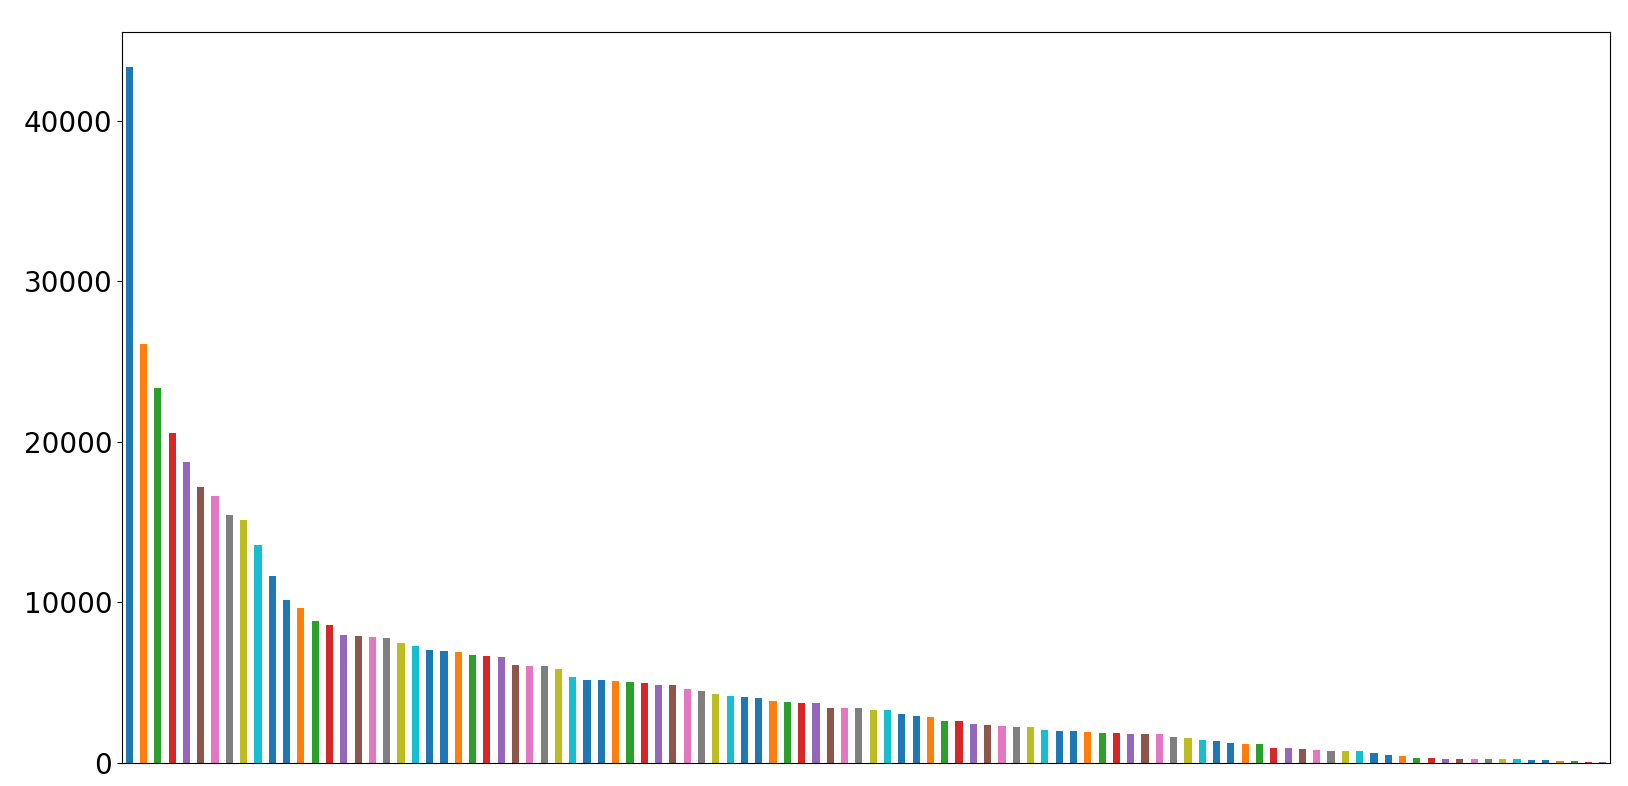
\includegraphics[width=\linewidth]{resources/InitialDistribution.png}
		\caption{A plot of the number of reviews per beer style}
		\label{fig:initialDistribution}
	\end{figure}

	The first step in preprocessing this dataset was to remove rows containing duplicates and missing values in the columns that are relevant for the experiment: beer style, text review. Next, some of the styles for which there wasn't a lot of data available were dropped, as they would be outliers for clustering. The threshold for this cut was chosen arbitrarily at 7000 reviews. 
	
	Upon inspection of the beer styles present in the dataset, a fine granularity was observed. For example, the difference between American Pale Ale and American India Pale Ale is minimal and not very rigorous. This and other similar cases would only confuse the classifier. For this reason, a mapping was made for each style to a broader category, using the taxonomy published by BusinessInsider\cite{BeerTaxonomy}. 
	
	The final mapping can be seen in figure \ref{fig:styleMapping}. Finally, a balanced dataset is built by selecting the minimum value for which we have an equal distribution of reviews per beer style, which is around 9500 per style. The analyzed dataset is made through random sampling of 9500 values for each of the remaining beer styles.
	
	\begin{figure}
		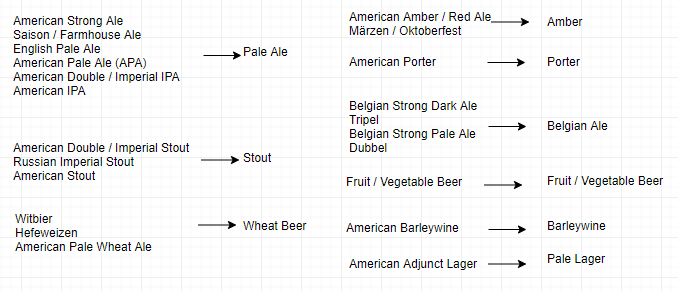
\includegraphics[width=\linewidth]{resources/MappingDiagram.png}
		\caption{Mapping of beer styles from the original dataset}
		\label{fig:styleMapping}
	\end{figure}
	
	
	\newpage
	\bibliography{references_document}
	\bibliographystyle{ieeetr}
\end{document}